\newpage
\section{Lorenz-Mie Form Factors for Static Light Scattering}
\label{sect:LorenzMieSLS}

Mie theory, also called Lorenz-Mie theory \cite{Mie1908,Hulst1957,Bohren1983},
is a complete mathematical-physical theory of the scattering of electromagnetic
radiation by spherical particles. Mie theory is named after its
developer German physicist Gustav Mie (1868 Rostock - 1957
Freiburg im Breisgau) and Danish physicist Ludvig Lorenz
(1829-1891) who independently developed the theory of
electromagnetic plane wave scattering by a dielectric sphere in
1908.

%In contrast to Rayleigh scattering or Dipole scattering, Mie
%scattering embraces all possible ratios of diameter to wavelength.
%It assumes an homogeneous, isotropic and optically linear material
%irradiated by an infinitely extending plane wave.

Mie scattering describes the scattering of electromagnetic
radiation by spherical particles of any size $r$, relative to the
wavelength, $\lambda$. Since the cases $r \ll \lambda$ and $r \gg
\lambda$ are covered by Rayleigh (dipole) scattering and geometric
scattering theories, respectively, Mie scattering often refers to
the case of $r \sim \lambda$.

%\cite{Mie1908}
%$^1$ Mie, G., Beitr�ge zur Optik tr�ber Medien, speziell kolloidaler Metall�sungen,
%Ann, Phys. (Leipzig), Vol. 25, 377-455, 1908. \\
%$^2$ H.C.\ van de Hulst, Light Scattering by Small Particles (Wiley, New York,
%1957), p. 70 \\
%$^3$ Craig F. Bohren and Donald R. Huffman, Absorption and
%Scattering of Light by Small Particles, (Wiley, New York, 1983),
%pp. 82�129.


\subsection{MieSphere}
\label{sect:MieSphere}
 ~\\

The Mie scattering formulae are given in several books (Van
de Hulst, 1957; Kerker, 1969; Deirmendjian, 1969) and by Dave
(1968a, 1969a), although not always in the forms most suited to
computation. The algorithm used here is based on the MIEV0 package
described in \cite{Wiscombe1979,Wiscombe1980}.
%\begin{enumerate}
%\item Wiscombe, W., 1979: Mie Scattering Calculations--Advances in
%Technique And Fast, Vector-Speed Computer Codes, Ncar Tech Note
%TN-140+STR, National Center For Atmospheric Research, Boulder,
%Colorado
%\item Wiscombe, W., 1980: Improved Mie scattering
%algorithms, Appl. Opt. 19, 1505-1509
%\end{enumerate}
The following input values are used:
\begin{align}
   \Theta &= 2\arcsin(Q\lambda/(4\pi)) \text{~with~} Q<Q_\text{max}=4\pi/\lambda  \nonumber \\
 R &= \text{radius of scattering sphere} \nonumber \\
 \lambda & = \text{wavelength of incident plane
 wave inside the solvent} \nonumber \\
m & = \text{complex refractive index of sphere relative to
surrounding medium} \nonumber \\
  & = m_\text{re} - i m_\text{im} \nonumber \\
  & \vert m \vert \geq 1 \text{~and~} m_\text{im} \geq 0 \nonumber \\
  & \text{or} \nonumber \\
  &  \vert m\vert  < 1 \text{~and~} m_\text{im} = 0 \nonumber \\
  \text{pol} & = 0 \text{~ unpolarized light} \nonumber \\
  \text{pol} & = 1 \text{~ parallel to scattering plane polarized light} \nonumber \\
  \text{pol} & = -1 \text{~ perpendicular to scattering plane polarized light} \nonumber
 \end{align}
 $\vert m\vert < 1$ would, for example, include visible light scattering from air
 bubbles in water.

\begin{figure}[htb]
\begin{center}
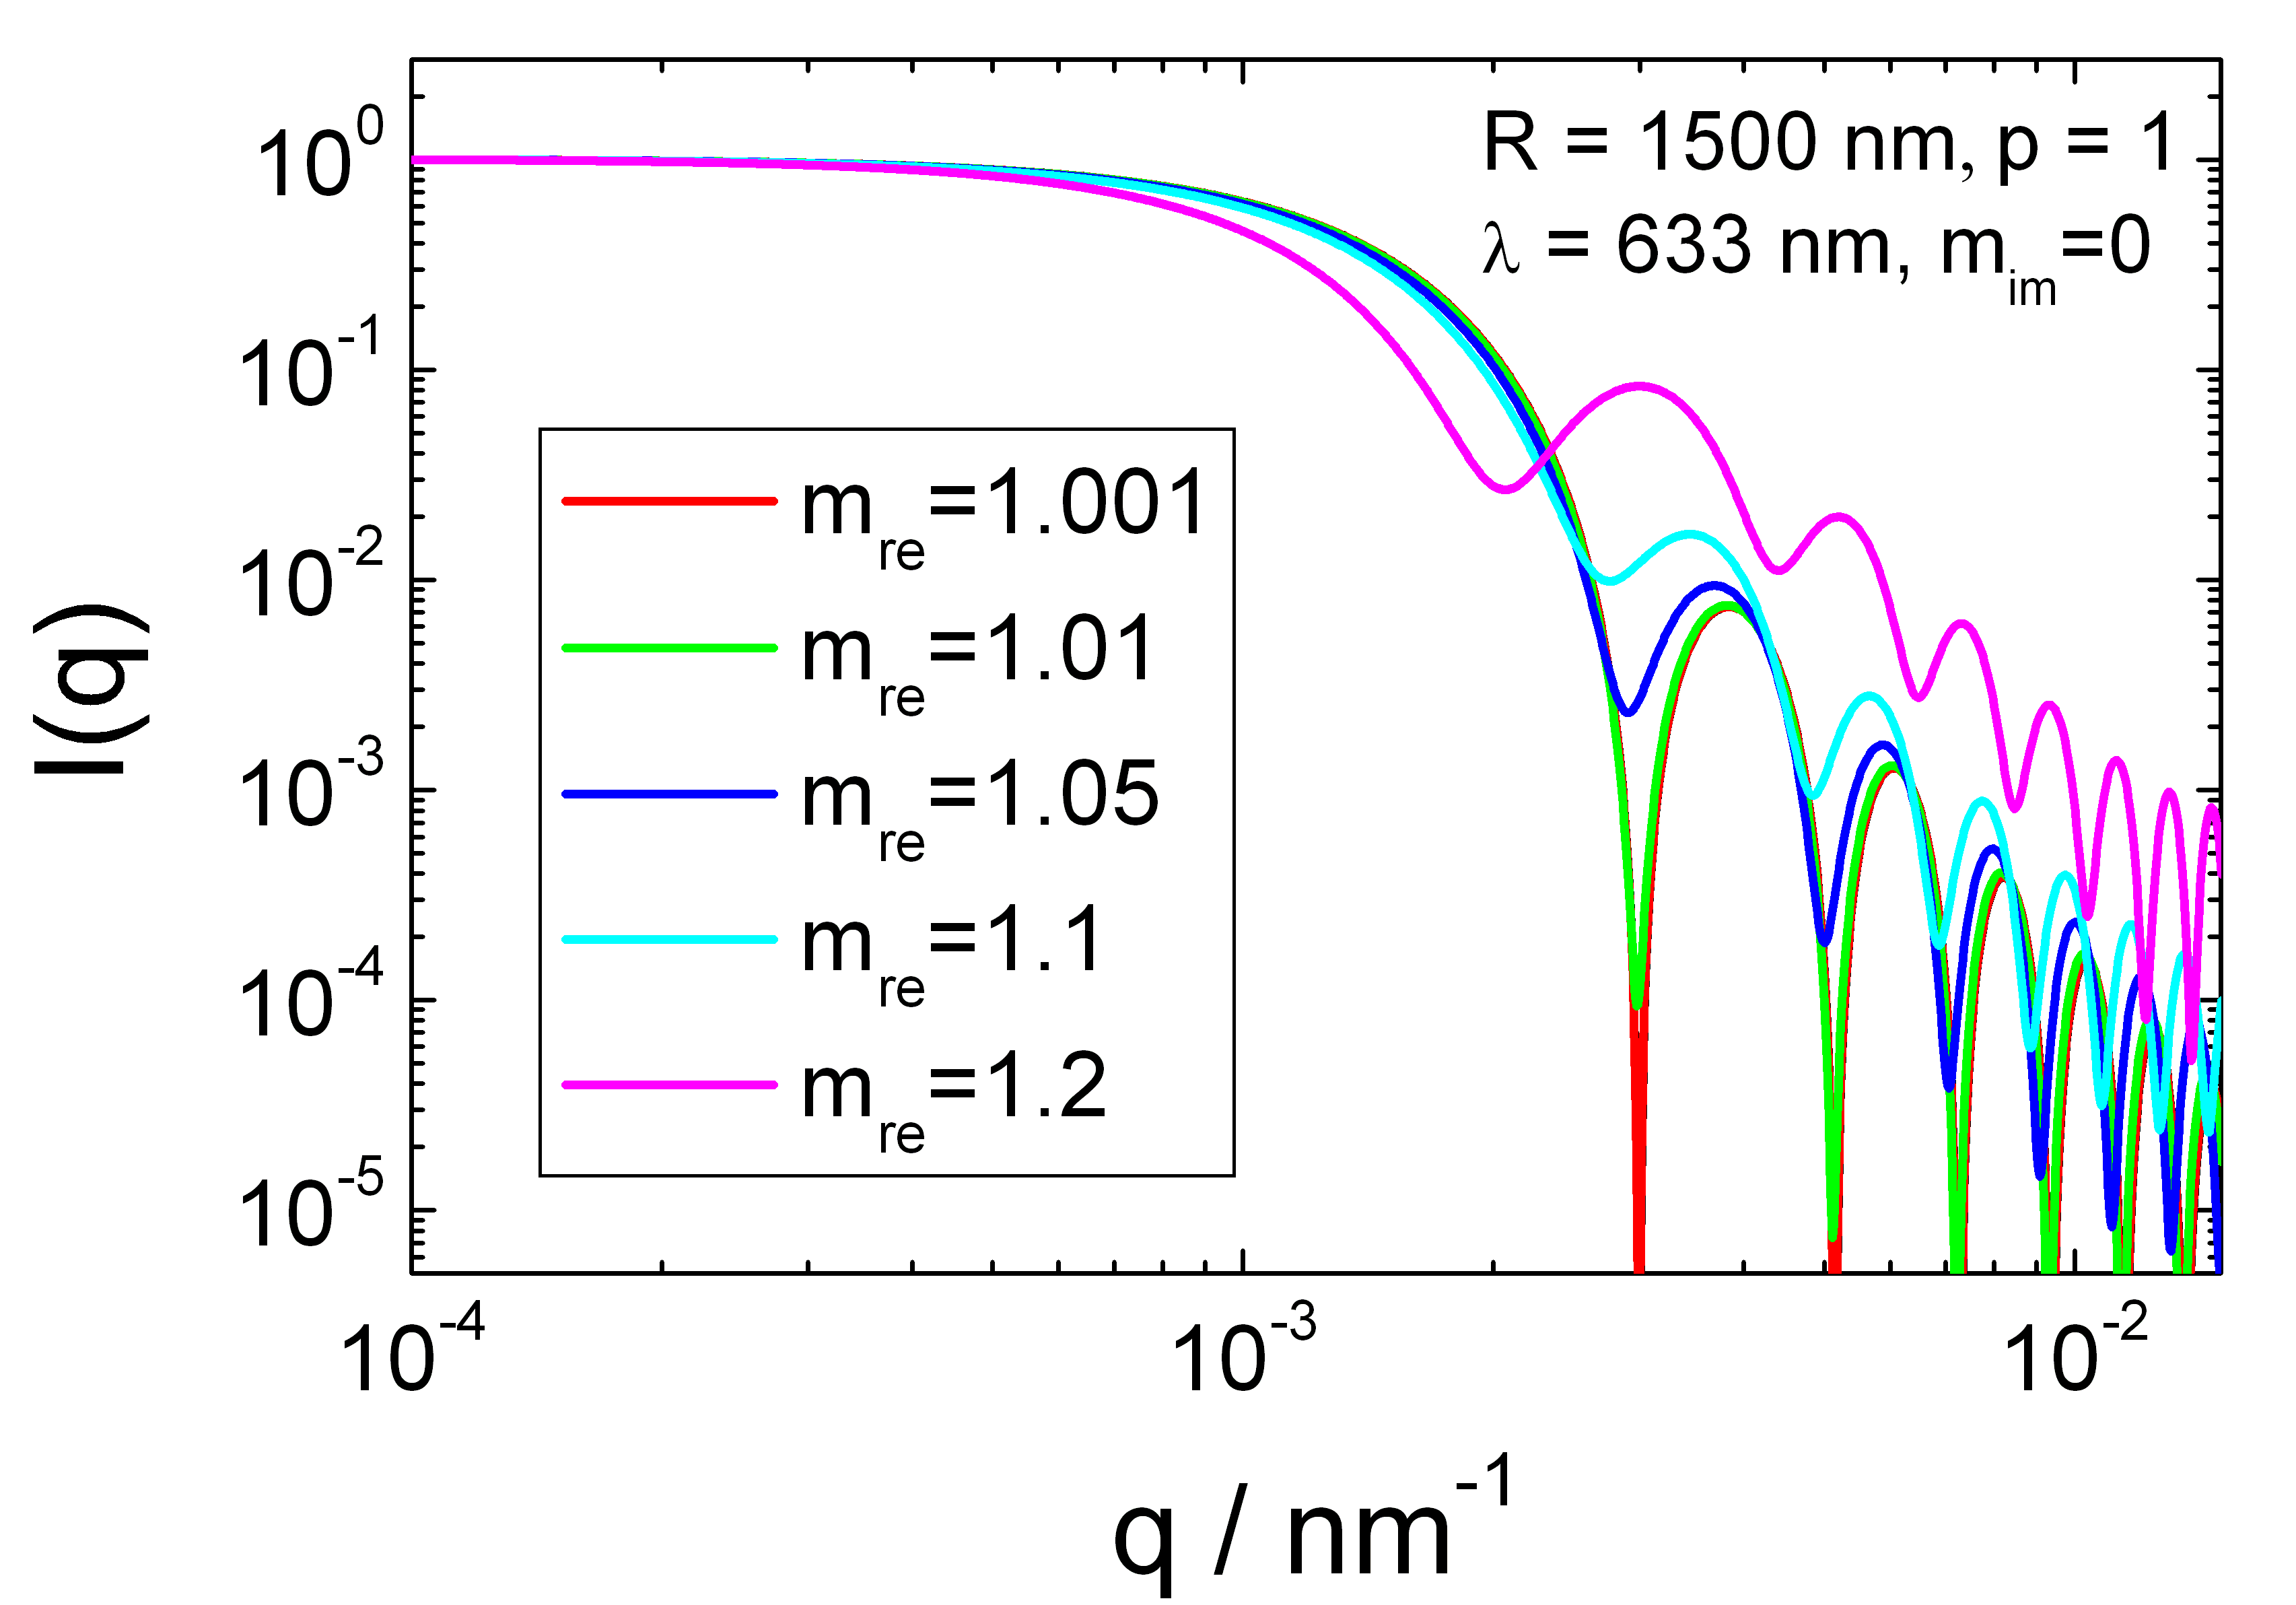
\includegraphics[width=0.65\textwidth,height=0.5\textwidth]{../images/form_factor/MieSphere/MieSphere.png}
\end{center}
\caption{Scattering intensity of a sphere using the formalism for Mie scattering.
The data are normalized to one for $q=0$. }
\label{fig:MieSphere}
\end{figure}

%%%%%%%%%%%%%%%%%%%%%%%%%%%%%%%%%%%%%%%%%%%%%%%%%%%%%%%%%%%%%%%%%%%%%%%%%%%%%%%%%%%

\clearpage
\subsection{MieShell}
\label{sect:MieShell}
~\\

This form factor is basing on the version of MieLay, which
computes electromagnetic scattering by a stratified sphere, i.e. a
particle consisting of a spherical core surrounded by a spherical
shell.  The surrounding medium is assumed to have refractive index
unity. The formulas, manipulated to avoid the ill-conditioning
that plagued earlier formulations, were published
in \cite{Toon1981}.
% Toon, O. and T. Ackerman, Applied Optics 20, 3657 (1981)\\
Further documentation, including definitons of input and
output  arguments, is inside the single precision version of this
program ({\tt SUBROUTINE MieLay}, available by anonymous ftp from
{\tt climate.gsfc.nasa.gov} in directory {\tt pub/wiscombe}). The
following input values are used:
\begin{align}
   \Theta &= 2\arcsin(Q\lambda/(4\pi)) \text{~with~} Q<Q_\text{max}=4\pi/\lambda  \nonumber \\
 R_\text{c} &= \text{radius of the core of scattering sphere} \nonumber \\
 R_\text{sh} &= \text{thickness of the shell of scattering sphere} \nonumber \\
 \lambda & = \text{wavelength of incident plane
 wave inside the solvent} \nonumber \\
m_\text{c} & = \text{complex refractive index of core relative to
surrounding medium} \nonumber \\
  & = m_\text{c,re} - i m_\text{c,im} \nonumber \\
  & \vert m_\text{c} \vert \geq 1 \text{~and~} m_\text{c,im} \geq 0 \nonumber \\
  & \text{or} \nonumber \\
  &  \vert m_\text{c}\vert  < 1 \text{~and~} m_\text{c,im} = 0 \nonumber \\
m_\text{s} & = \text{complex refractive index of core relative to
surrounding medium} \nonumber \\
  & = m_\text{s,re} - i m_\text{s,im} \nonumber \\
  \text{pol} & = 0 \text{~ unpolarized light} \nonumber \\
  \text{pol} & = 1 \text{~ parallel to scattering plane polarized light} \nonumber \\
  \text{pol} & = -1 \text{~ perpendicular to scattering plane polarized light} \nonumber
 \end{align}
 $\vert m\vert < 1$ would, for example, include visible light scattering from air
 bubbles in water.


\begin{figure}[htb]
\begin{center}
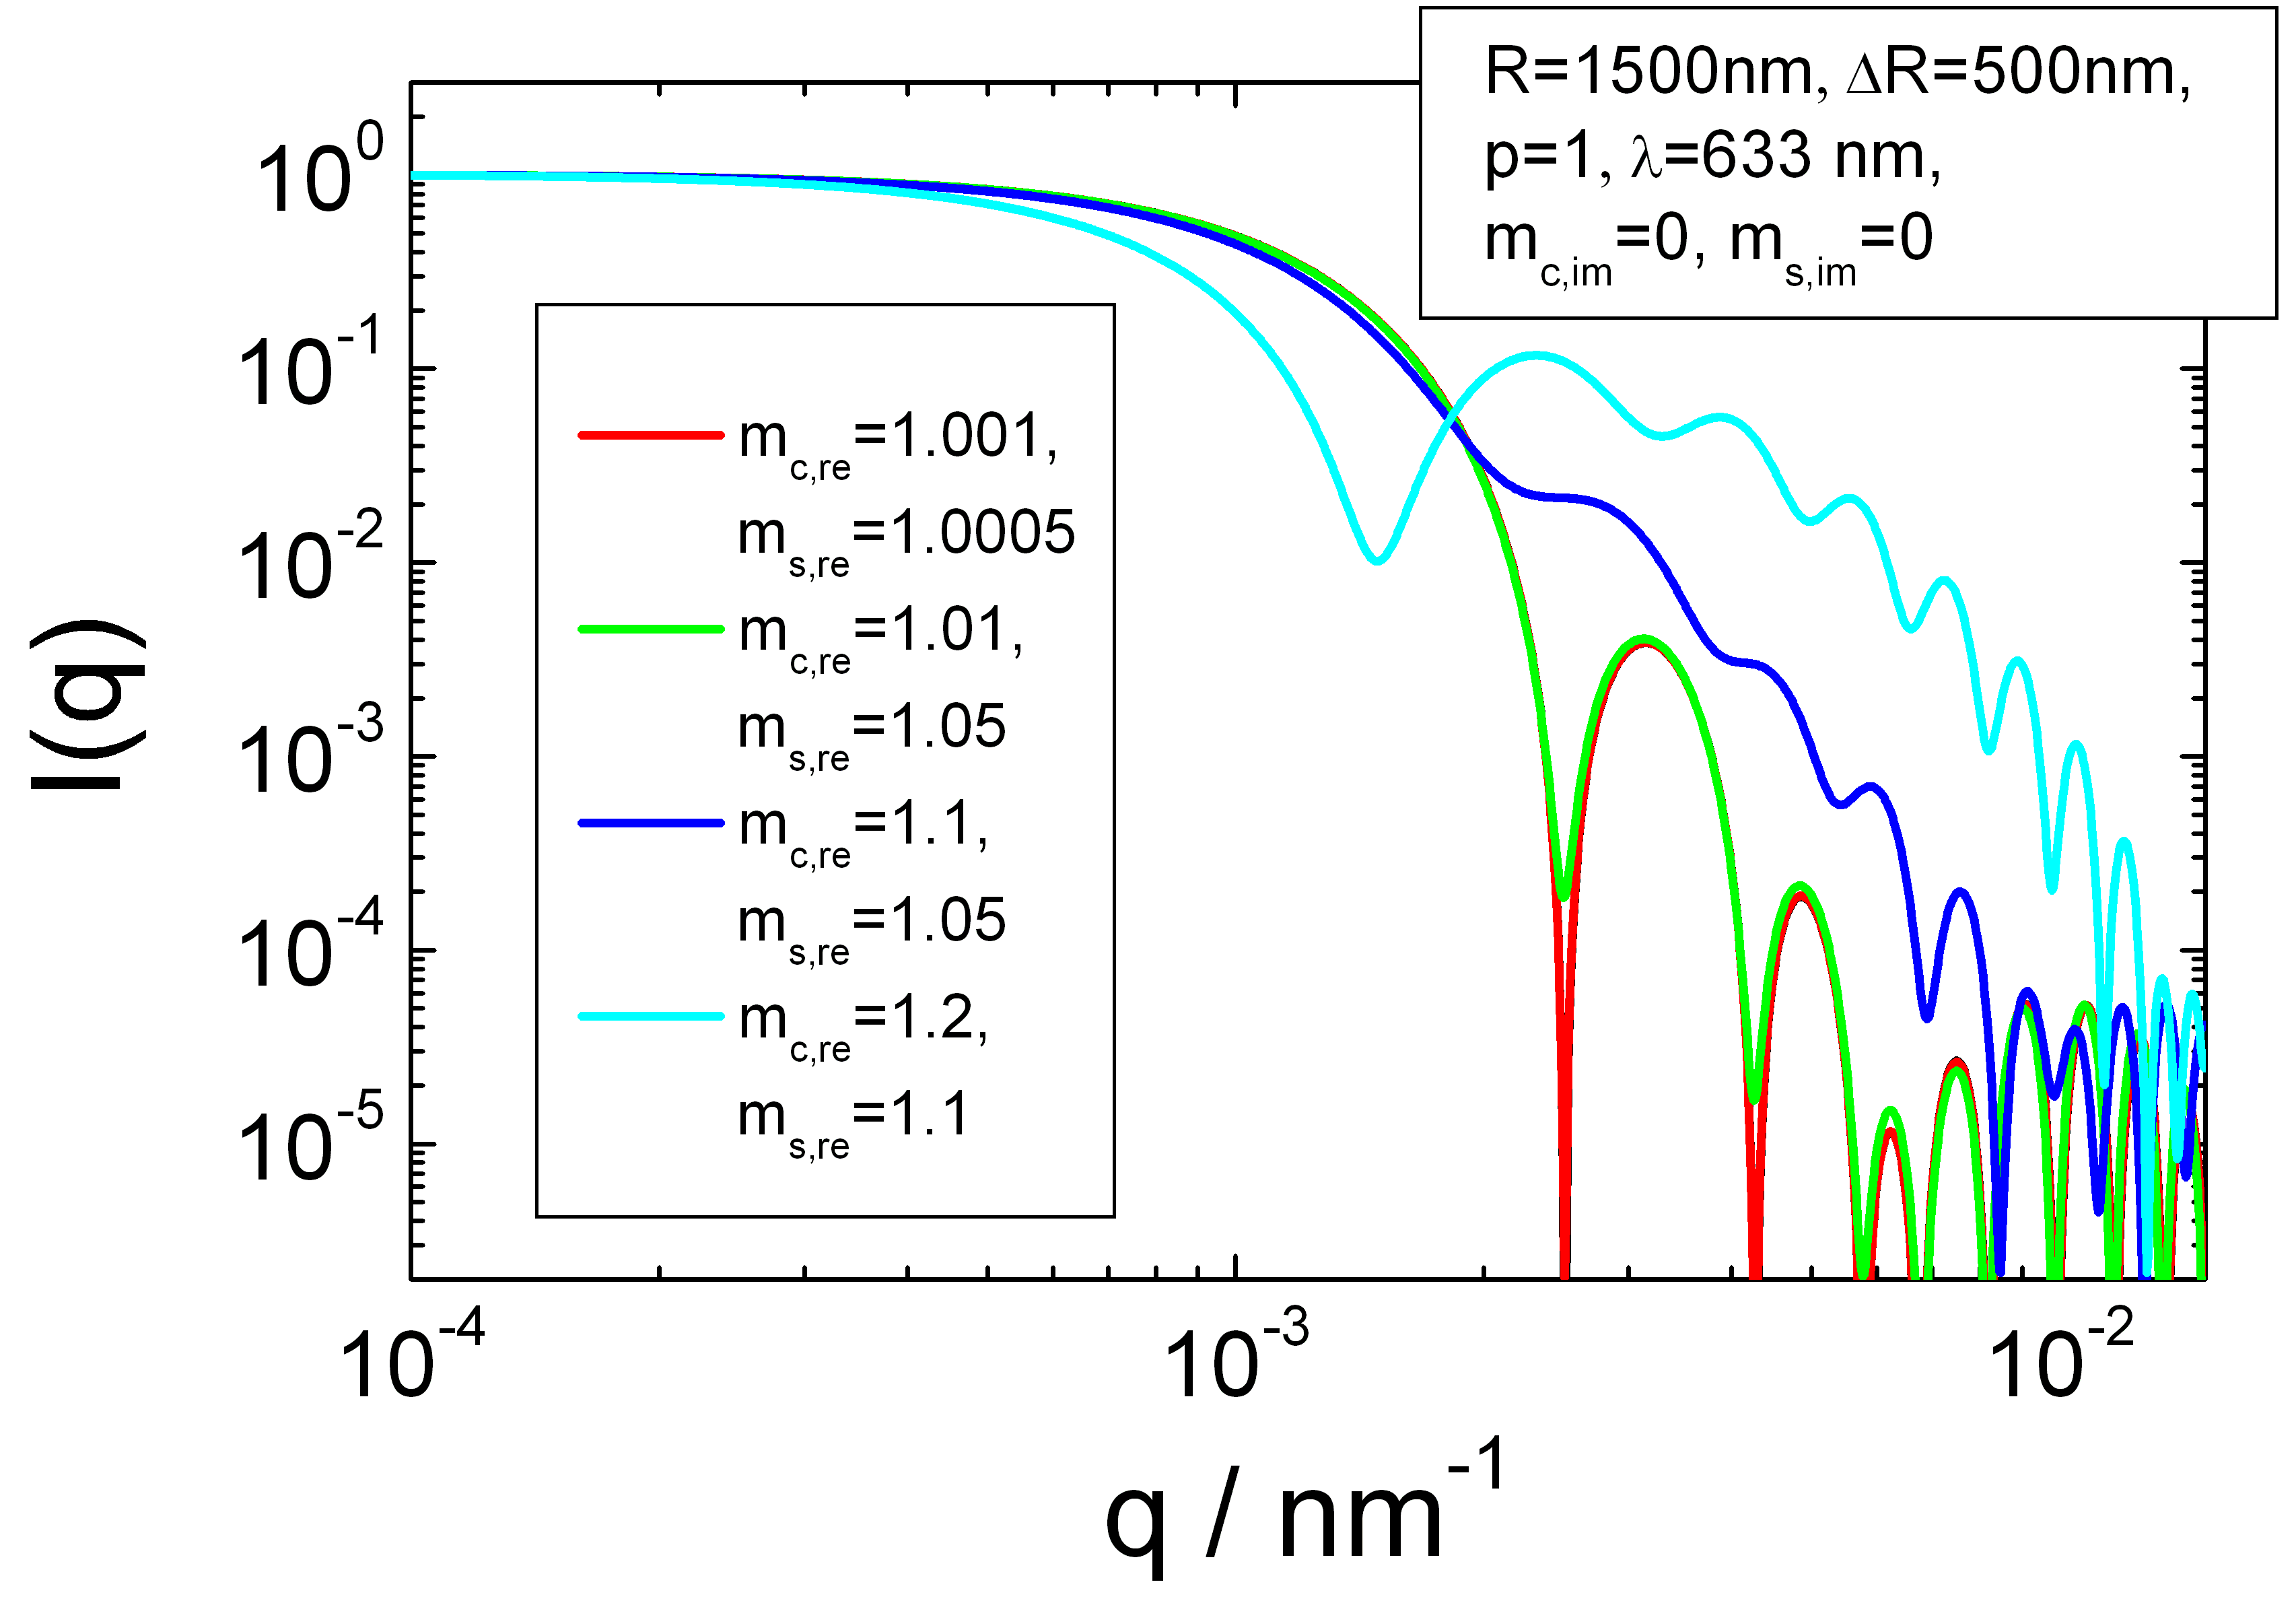
\includegraphics[width=0.65\textwidth,height=0.5\textwidth]{../images/form_factor/MieSphere/MieShell.png}
\end{center}
\caption{Scattering intensity of a spherical shell using the formalism for Mie scattering.
The data are normalized to one for $q=0$. }
\label{fig:MieShell}
\end{figure}
